\documentclass{sig-alternate}
\usepackage{textcomp}
\usepackage{graphics}
\pagestyle{plain}
\usepackage{subfigure}
\usepackage[margin=10pt,font=small,labelfont=bf, labelsep=endash, skip=0pt]{caption}
\usepackage[latin1]{inputenc}
\usepackage{listings}

\begin{document}

\pagenumbering{arabic}

\title{Mahjong Solitaire}
\subtitle{Sistemas de Inteligencia Artifical - ITBA}

\numberofauthors{3}

\author{
	\alignauthor{Carlos Sessa}\\
	\alignauthor{Lucas Pizzagalli}\\
	\alignauthor{Nicol\'as Purita}\\
}

\date{09 de Mayo de 2011}

\maketitle

\section*{Introducci\'on}
	Se implementa un \textit{Sistema de Producci\'on} el cual es utilizado para resolver un juego denominado \textbf{Mahjong-Solitaire}, tambien conocido como el \textit{Taipei}. Se utiliza un motor de inferencia en \textit{Java} para la resoluci\'on del problema designado, el cual fue entregado por la c\'atedra. \\
	Como punto de partida para crear el \textit{Sistema de Producci\'on} se dise\~{n}a un sistema de almacenamiento apropiado que represente el problema de la forma m\'as \'optima. Se utilizan 3 estrat\'egias de b\'usqueda no informadas para comparar las distintas soluciones alcanzadas, las cuales se detallan en el transcurso del informe

\section*{Reglas del Mahjong-Solitaire}
	El juego \textbf{Mahjong-Solitaire} consiste en eliminar todas las fichas de un tablero de 144 fichas. \\
	Una ficha puede ser removida siempre que no se encuentre bloqueada y ademas cumpla con la condici\'on de que las fichas son del mismo tipo. La cantidad y tipos de fichas se encuentra definido, como lo muestra la Figura \ref{fig:tiles}. Existe una excepci\'on en la remoci\'on de las fichas del tipo \textit{Season} o \textit{Flowers}. La excepci\'on esta basada en que cualquier par de fichas \textit{Season} o \textit{Flowers} puede ser removidas utilizando cualquier combinaci\'on entre las mismas, esto se debe a que existen unicamente 4 fichas de cada tipo. \\
	Una ficha bloqueada puede estar en forma \textit{Horizontal}, \textit{Vertical} o \textit{Ambos}. Estos bloqueos se definen del siguiente modo:
	\begin{itemize}
		\item \textbf{Horizontal}: La ficha elegida posee una ficha a su izquierda y derecha.
		\item \textbf{Vertical}: La ficha elegida posee una ficha encima de ella.		
	\end{itemize}
	
\section*{Desarrollo}

	Se representa un estado del juego como un vector de vectores en donde cada celda posee una \textit{Tile}. Esta vector de vectores es del tipo:
	\begin{itemize}
		\item \textit{Tile}[a][b][c]
	\end{itemize}
	donde \textit{a} indica el nivel en el que se encuentra la ficha, \textit{b} es la fila donde se encuentra y \textit{c} la columna. La clase \textit{Tile} esta definida como la composici\'on de un tipo de ficha y un n\'umero.
	
\section*{Funciones de costo}

	Dado que el objetivo del juego es simplemente retirar todas las fichas del tablero, la funci\'on de costo propuesta es la cantidad de fichas sacadas en cada estado. \\
	Esta funci\'on de costo es variable si buscamos la soluci\'on utilizando un ordenador, dado que se pueden aplicar varias reglas en simult\'aneo seg\'un un criterio de selecci\'on de pares de fichas. \\
	Caso contrario de esta funci\'on de costo en la vida real ya que en cada estado del juego se pueden remover unicamente 2 fichas en simult\'aneo, por lo tanto esta funci\'on se comporta en forma constante.

\section*{Heur\'isticas}



\section*{Resultados y Conclusiones}	

\onecolumn
\begin{figure}[h!]
  \begin{center}
  	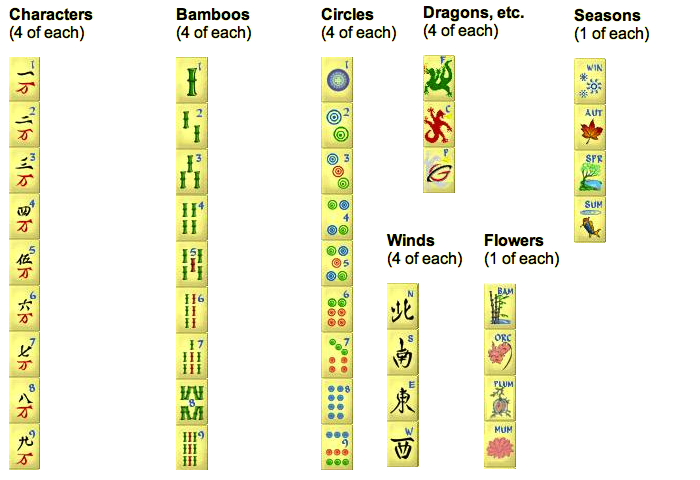
\includegraphics[scale=0.5]{images/tiles.png}
  \end{center}
  \caption{Distribuci\'on de fichas.}
  \label{fig:tiles}
\end{figure}
\end{document}